\section{Cost, Schedule and Risks}


%%%%%%%%%%%%%%%%%%%%%%%%%%%%
%\subsection{Logistics Cost and Schedule} %, and Risk Analysis}
%\label{sec:fdsp-tc-log-cost}

The costs for the logistics activities and facilities are the responsibility of \dword{lbnf} and Fermilab's \dword{sdsd}, and therefore are not listed here. %  is not a DUNE responsibility and will be covered as part of the host laboratory responsibilities.

According to the overall \dword{lbnf} and \dword{dune} schedule, the \dword{aup} for \dword{lbnf} (post-\dword{cf}) and \dword{dune} teams to the north cavern and \dword{cuc} is \cucbenocc{}.

The  \dword{sdwf} will be in place approximately one year before the warm structure installation begins, i.e., in fall 2021.  Extra storage must be available before  this facility is ready  since  \dword{apa}s, \dword{cuc} infrastructure, and equipment all begin arriving in South Dakota during summer 2021.  As an interim solution, we plan to store these early items at \dword{fnal} until the \dword{sdwf} is ready.

Figure \ref{fig:high-level-schedule} shows the overview of the schedule for the main activities for \dword{detmodule} \#1. 


%%%%%%%%%%%%%%%%%%%%%%%%%%%%
\subsection{FROM ITF FILE: Cost, Schedule and Risk Analysis}
\label{sec:fdsp-tc-itf-cost}

\fixme{Add costs when they are available (Anne adds 3/25: Cost table template coming soon; do not add any numbers yet.)}

%%%%%%%%%%%%%%%
\subsection{FROM ITF FILE: Timeline and APA Integration Schedule}

\fixme{Anne adds new standard schedule table 3/25, table~\ref{tab:sp-iic-sched}. Leave orange (dunepeach) lines as they are, add your milestones around them.}

%This is a standard table template for the TDR schedules.  It contains overall FD dates from Eric James as of March 2019 (orange) that are held in macros in the common/defs.tex file so that the TDR team can change them if needed. Please do not edit these lines! Please add your milestone dates to fit in with the overall FD schedule. 


\begin{dunetable}
[\dword{sp} Installation, Integration, and Commissioning Schedule]
{p{0.65\textwidth}p{0.25\textwidth}}
{tab:sp-iic-sched}
{\dword{sp} Installation, Integration, and Commissioning Schedule}   
Milestone & Date (Month YYYY)   \\ \toprowrule
Technology Decision Dates &      \\ \colhline
Final Design Review Dates &      \\ \colhline
Start of module 0 component production for ProtoDUNE-II &      \\ \colhline
End of module 0 component production for ProtoDUNE-II &      \\ \colhline
\rowcolor{dunepeach} Start of \dword{pdsp}-II installation& \startpduneiispinstall      \\ \colhline
\rowcolor{dunepeach} Start of \dword{pddp}-II installation& \startpduneiidpinstall      \\ \colhline
 \dword{prr} dates &      \\ \colhline
Start of  (component 1) production  &      \\ \colhline
Start of (component 2) production  &      \\ \colhline
Start of  (component 3) production  &      \\ \colhline
\rowcolor{dunepeach}South Dakota Logistics Warehouse available& \sdlwavailable      \\ \colhline
\rowcolor{dunepeach}Beneficial occupancy of cavern 1 and \dword{cuc}& \cucbenocc      \\ \colhline
\rowcolor{dunepeach} \dword{cuc} counting room accessible& \accesscuccountrm      \\ \colhline
\rowcolor{dunepeach}Top of \dword{detmodule} \#1 cryostat accessible& \accesstopfirstcryo      \\ \colhline
End of  (component 1) production  &      \\ \colhline
... & ...                       \\ \colhline
\rowcolor{dunepeach}Start of \dword{detmodule} \#1 TPC installation& \startfirsttpcinstall      \\ \colhline
\rowcolor{dunepeach}End of \dword{detmodule} \#1 TPC installation& \firsttpcinstallend      \\ \colhline
\rowcolor{dunepeach}Top of \dword{detmodule} \#2 accessible& \accesstopsecondcryo      \\ \colhline
 \rowcolor{dunepeach}Start of \dword{detmodule} \#2 TPC installation& \startsecondtpcinstall      \\ \colhline
\rowcolor{dunepeach}End of \dword{detmodule} \#2 TPC installation& \secondtpcinstallend      \\ \colhline

last item & ...                         \\
\end{dunetable}


%The timeline for starting up the \dword{itf} is late 2022 when \dwords{pd} and \dword{ce} are available to integrate into the \dword{apa}s.  This is two years before installation begins. This schedule has the advantage of allowing all integrated components to be tested as soon as possible and minimizing any schedule risk if problems occur. However $3/4$ of the \dword{apa} are produced before the first \dword{ce} module is available for the risk reduction applies primarily to the electronics. The integration team size is smaller than what would be required underground as the work proceeds over a longer time. 
The integration area underground must be ready to start operations when the \dwords{pd} and \dword{ce}  become available in late 2022; this is after three quarters of the \dword{apa}s are produced and two years before installation begins.  This schedule allows the \dword{ce} to be tested and integrated soon after production, thus minimizing the schedule risk in the case of unanticpated problems. This risk reduction applies primarily to the electronics. %The integration team size is smaller than what would be required underground as the work proceeds over a longer time. 

%Using four work stations and working with only a day shift, installing  an \dword{apa} pair should take approximately nine shifts as shown in Figure \ref{fig:ITF-Schedule}. The 150 \dword{apa} then require 270 work days.
Integrating two \dword{apa}s (to make a top-bottom pair) %that will be shipped together) 
is expected to take approximately nine shifts as shown in Figure \ref{fig:ITF-Schedule}. Using four work stations and working only day shifts, the 150 \dword{apa} pairs then require 270 work days.  

\begin{dunefigure}[Schedule for APA integration]
{fig:ITF-Schedule}
    {Schedule for APA integration}
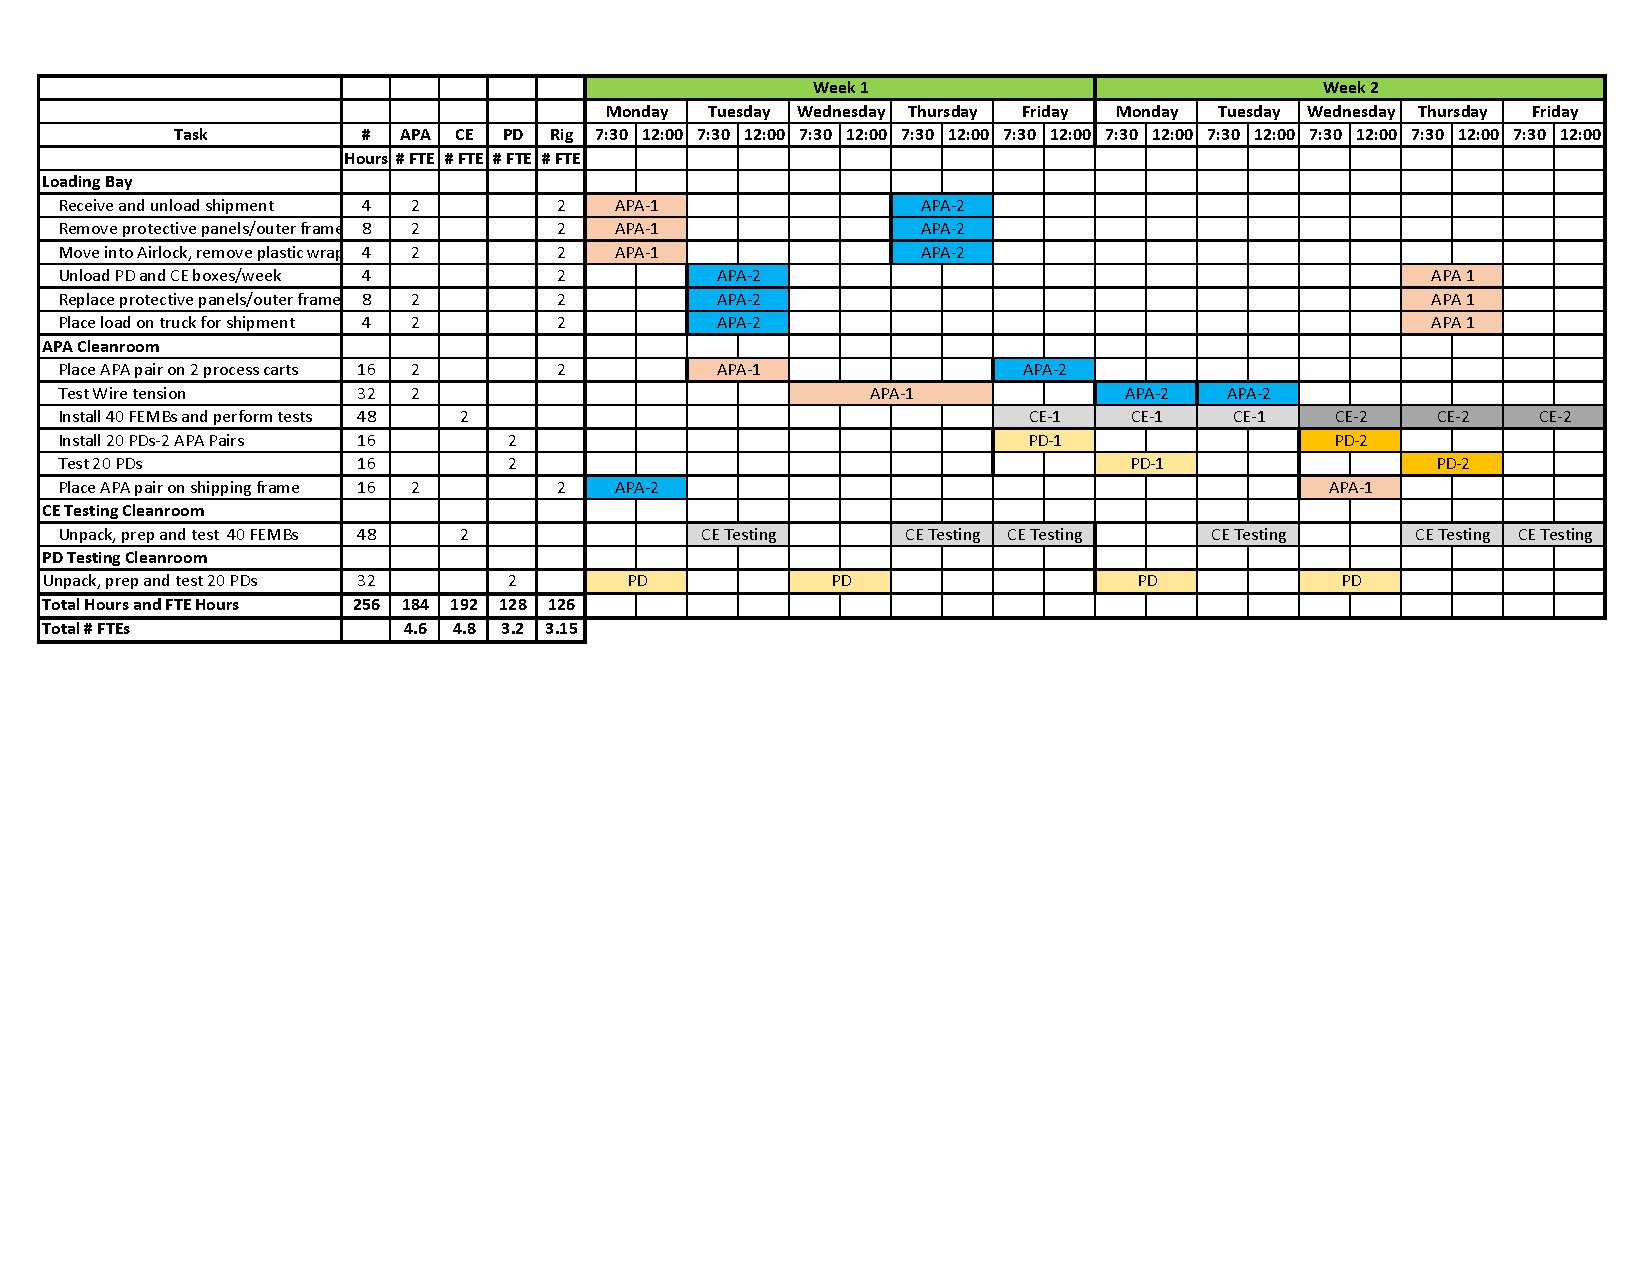
\includegraphics[width=0.98\textwidth]
{ITF-Schedule.pdf} 
\end{dunefigure}


\fixme{A graphical representation of the schedule is used instead of the template as the duration and relative timing of the work is critical for the installation. Jim}

%%%%%%%%%%%%%%%%%%%%%%%%%%%%
\subsection{FROM INFRASTRUCTURE FILE Costs, Schedule, and Risk Analysis}
\label{sec:fdsp-tc-infr-cost}

\fixme{Add costs when available -- (anne) probably want only one cost and risk table in chapter; not sure about schedule since you have special gantt charts}

{\bf Installation Setup Phase:} %This is a more difficult phase to schedule and may be adjusted often with multiple projects going forward at once. The \dword{cf} work is basically completed, which reduces the number of \dwords{fte} underground, allowing us to begin the installation infrastructure. We begin two 10 hour shifts per day as the work ramps up.  Once the cold cryostat is approximately six months into the installation schedule, floor space becomes available in the north cavern. The \coldbox construction must be started ASAP because the welding takes approximately six months. In parallel to this, the machine shop area can be set up and the bridge between the north and south sides of the cavern can be constructed.  Once the bridge is completed, work on the assembly crane, \dword{apa} cabling tower, \dword{apa} assembly tower, and \dword{cpa} assembly station can begin. 
    This is a more difficult phase to schedule and may require frequent adjustment, with multiple projects going forward at once. The \dword{cf} work is essentially completed by this point, which reduces the number of \dwords{fte} underground, allowing us to begin the installation infrastructure. 
    \fixme{Sort of a non sequitur. Reduced cf FTEs allows you to have more FTEs, but it's not clear that it's what allows you to begin the installation infra } We begin two ten-hour shifts per day as the work ramps up.  Once the  cryostat cold structure is approximately six months into the installation schedule, floor space becomes available in the north cavern. The \coldbox construction must begin immediately at this point because the welding takes approximately six months. In parallel, the machine shop area can be set up and the bridge between the north and south sides of the cavern can be constructed.  Once the bridge is completed, work on the assembly crane, \dword{apa} cabling tower, \dword{apa} assembly tower, and \dword{cpa} assembly station can begin. 
    
%Installation of the detector support system could begin during the final installation stages of the cryostat cold structure because they both require full height scaffolding for all the welding on the top of the cryostat. This was how the \dword{protodune} \dword{dss} was installed. The details have not yet been worked out with the contractor, so work may be done in stages. This requires a crew on top of the cryostat installing the \dword{dss} support feedhroughs from the top of the cryostat as shown in Figure \ref{fig:install-dss-feedthru}. 
Installation of the \dword{dss} could begin during the final installation stages of the cryostat cold structure because they both require full-height scaffolding for the welding on the top of the cryostat. The \dword{protodune} \dword{dss} was installed this way. This requires a crew on top of the cryostat installing the \dword{dss} support feedhroughs from the top, as shown in Figure~\ref{fig:install-dss-feedthru}.  The details have not yet been worked out with the contractor, so work may be done in stages. 

A detailed schedule of the installation infrastructure time period is shown in Figure~\ref{fig:Installation_Infrastructure_Schedule}.
    
\begin{dunefigure}[Schedule for the infrastructure installation]
{fig:Installation_Infrastructure_Schedule}
    {Schedule for the infrastructure installation}
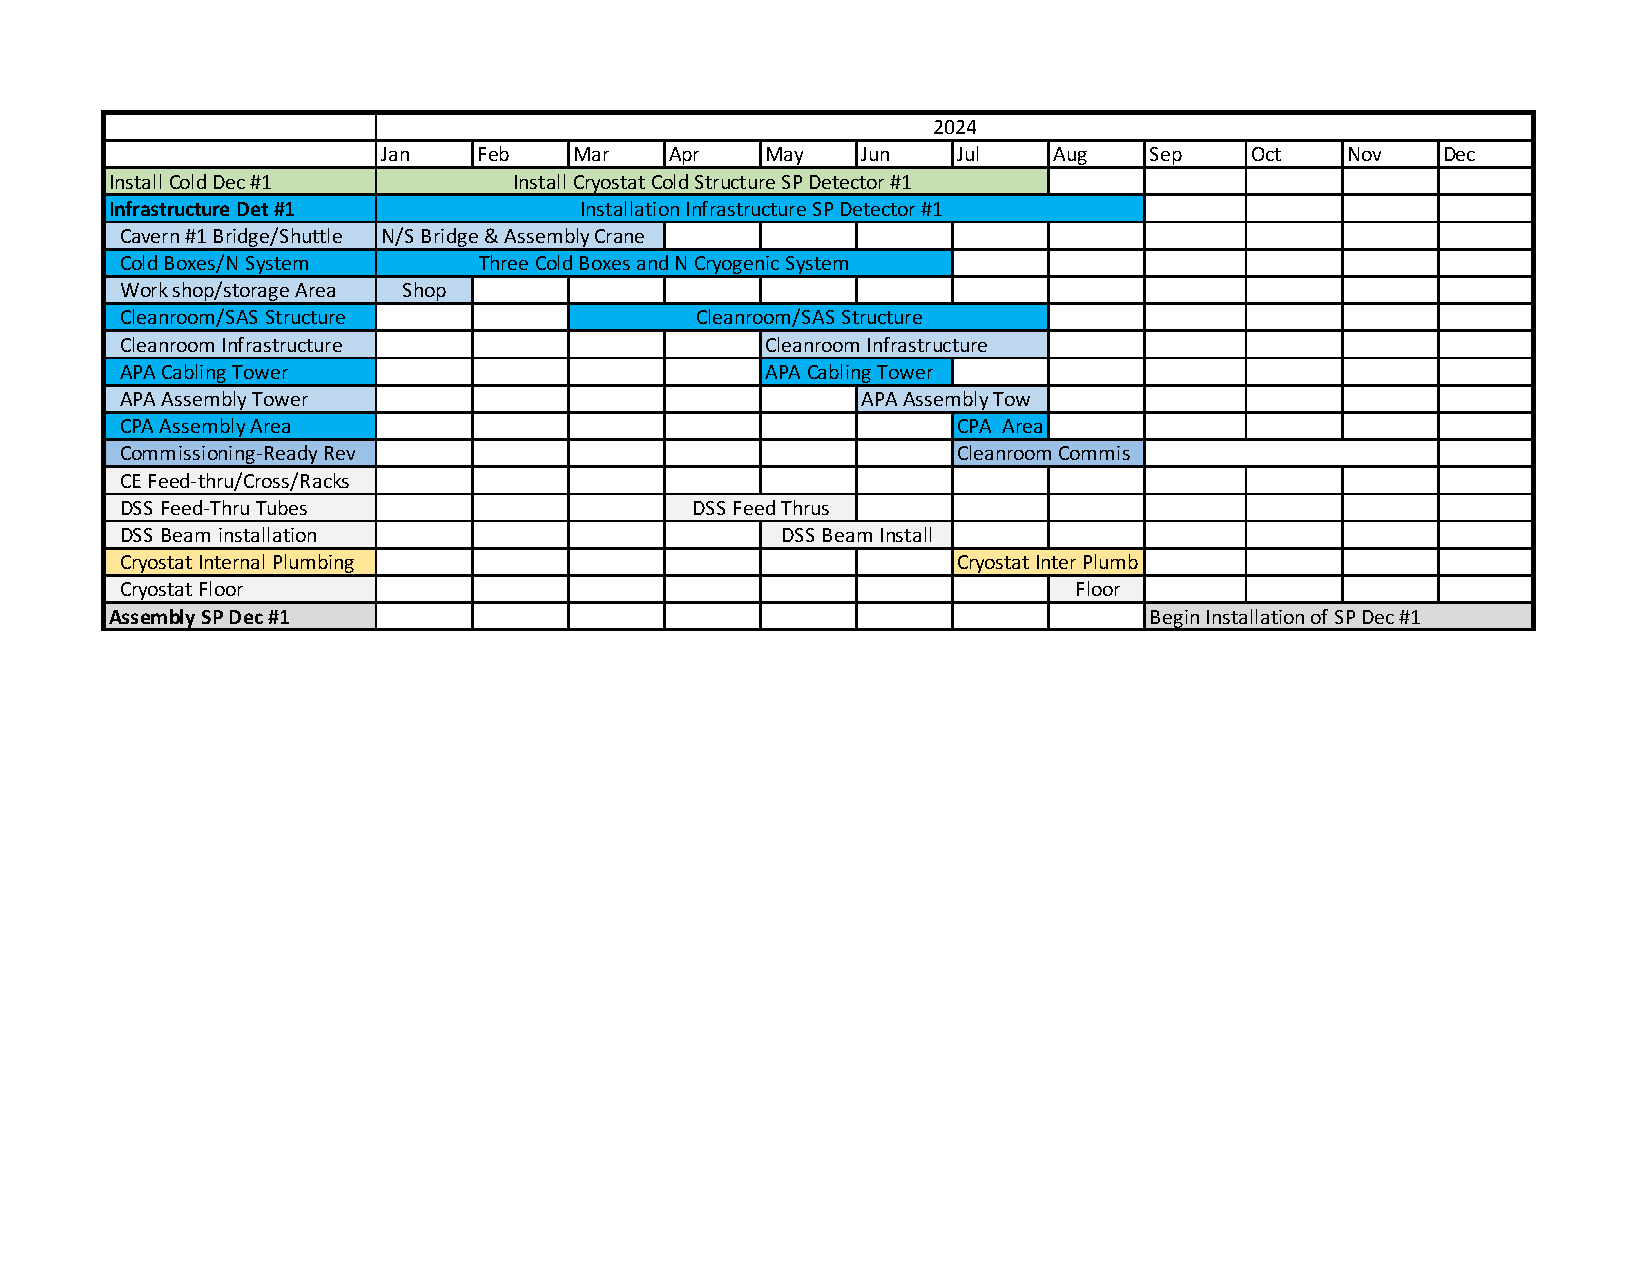
\includegraphics[width=0.98\textwidth]
{Installation_Infrastructure_Schedule} 
\end{dunefigure}

\fixme{A graphical representation of the schedule is used since it is critical to convey the time sequencing and how the work is overlapping. Jim }

% clear the figure buffer before starting the next section
\clearpage

%%%%%%%%%%%%%%%%%%%%%%%%

%%%%%%%%%%%%%%%%%%%%%%%%%%%%
\subsection{Costs and Schedule}
\label{sec:fdsp-tc-inst-cost}

\fixme{Jim S to rework this section}

\fixme{I just added the template for the Cost table. Fill in 1st column with the cost items but leave the cost and hours columns empty for now.  Risks to be treated like specs -- still to come. (Anne) }

\begin{dunetable}
[Cost Summary]
{p{0.5\textwidth}p{0.2\textwidth}p{0.2\textwidth}}
{tab:XXcostsumm}
{Cost Summary}   
Cost Item & M\&S (k\$ US) & Labor Hours \\ \toprowrule
\rowcolor{dunepeach} Design, Engineering and R\&D &  &     \\ \colhline
 (E.g., Photosensors design) &     &             \\ \colhline
 (E.g., Mechanics design) &     &             \\ \colhline
 &     &             \\ \colhline
 &     &             \\ \colhline
 &     &             \\ \colhline
 &     &             \\ \colhline
\rowcolor{dunepeach} Production Setup &  &     \\ \colhline
 (E.g., Photosensors production setup)  &     &             \\ \colhline
 &     &             \\ \colhline 
 &     &             \\ \colhline
 &     &             \\ \colhline 
 &     &             \\ \colhline
 &     &             \\ \colhline
\rowcolor{dunepeach} Production &  &     \\ \colhline
 (E.g., Photosensors production)  &     &             \\ \colhline
 &     &             \\ \colhline 
 &     &             \\ \colhline
 &     &             \\ \colhline 
 &     &             \\ \colhline
 &     &             \\ \colhline
\rowcolor{dunepeach} DUNE FD Integration \& Installation  &  &     \\ \colhline
 &     &             \\ \colhline
 &     &             \\ \colhline 
 &     &             \\ \colhline
 &     &             \\ \colhline 
 &     &             \\ \colhline
 (last line) &     &             \\
\end{dunetable}


The schedule for the \dword{spmod} 1 Installation is a complicated dance relying on many entities including \dword{cf}, \dword{lbnf}, and \dword{sdsta}.  The maximum number of people allowed underground is 144 which is the number of people that can be evacuated in one hour.  This is particularly critical during the excavation of Cavern 3. Different underground areas will allow access at different times, so a detailed summary of these times are shown in Figure~\ref{fig:Overview-of-SinglePhase-Schedule}. 



\begin{dunefigure}[Overview of the single-phase schedule]
{fig:Overview-of-SinglePhase-Schedule}
{Schedule Overview of the Single Phase Detector \#1}                
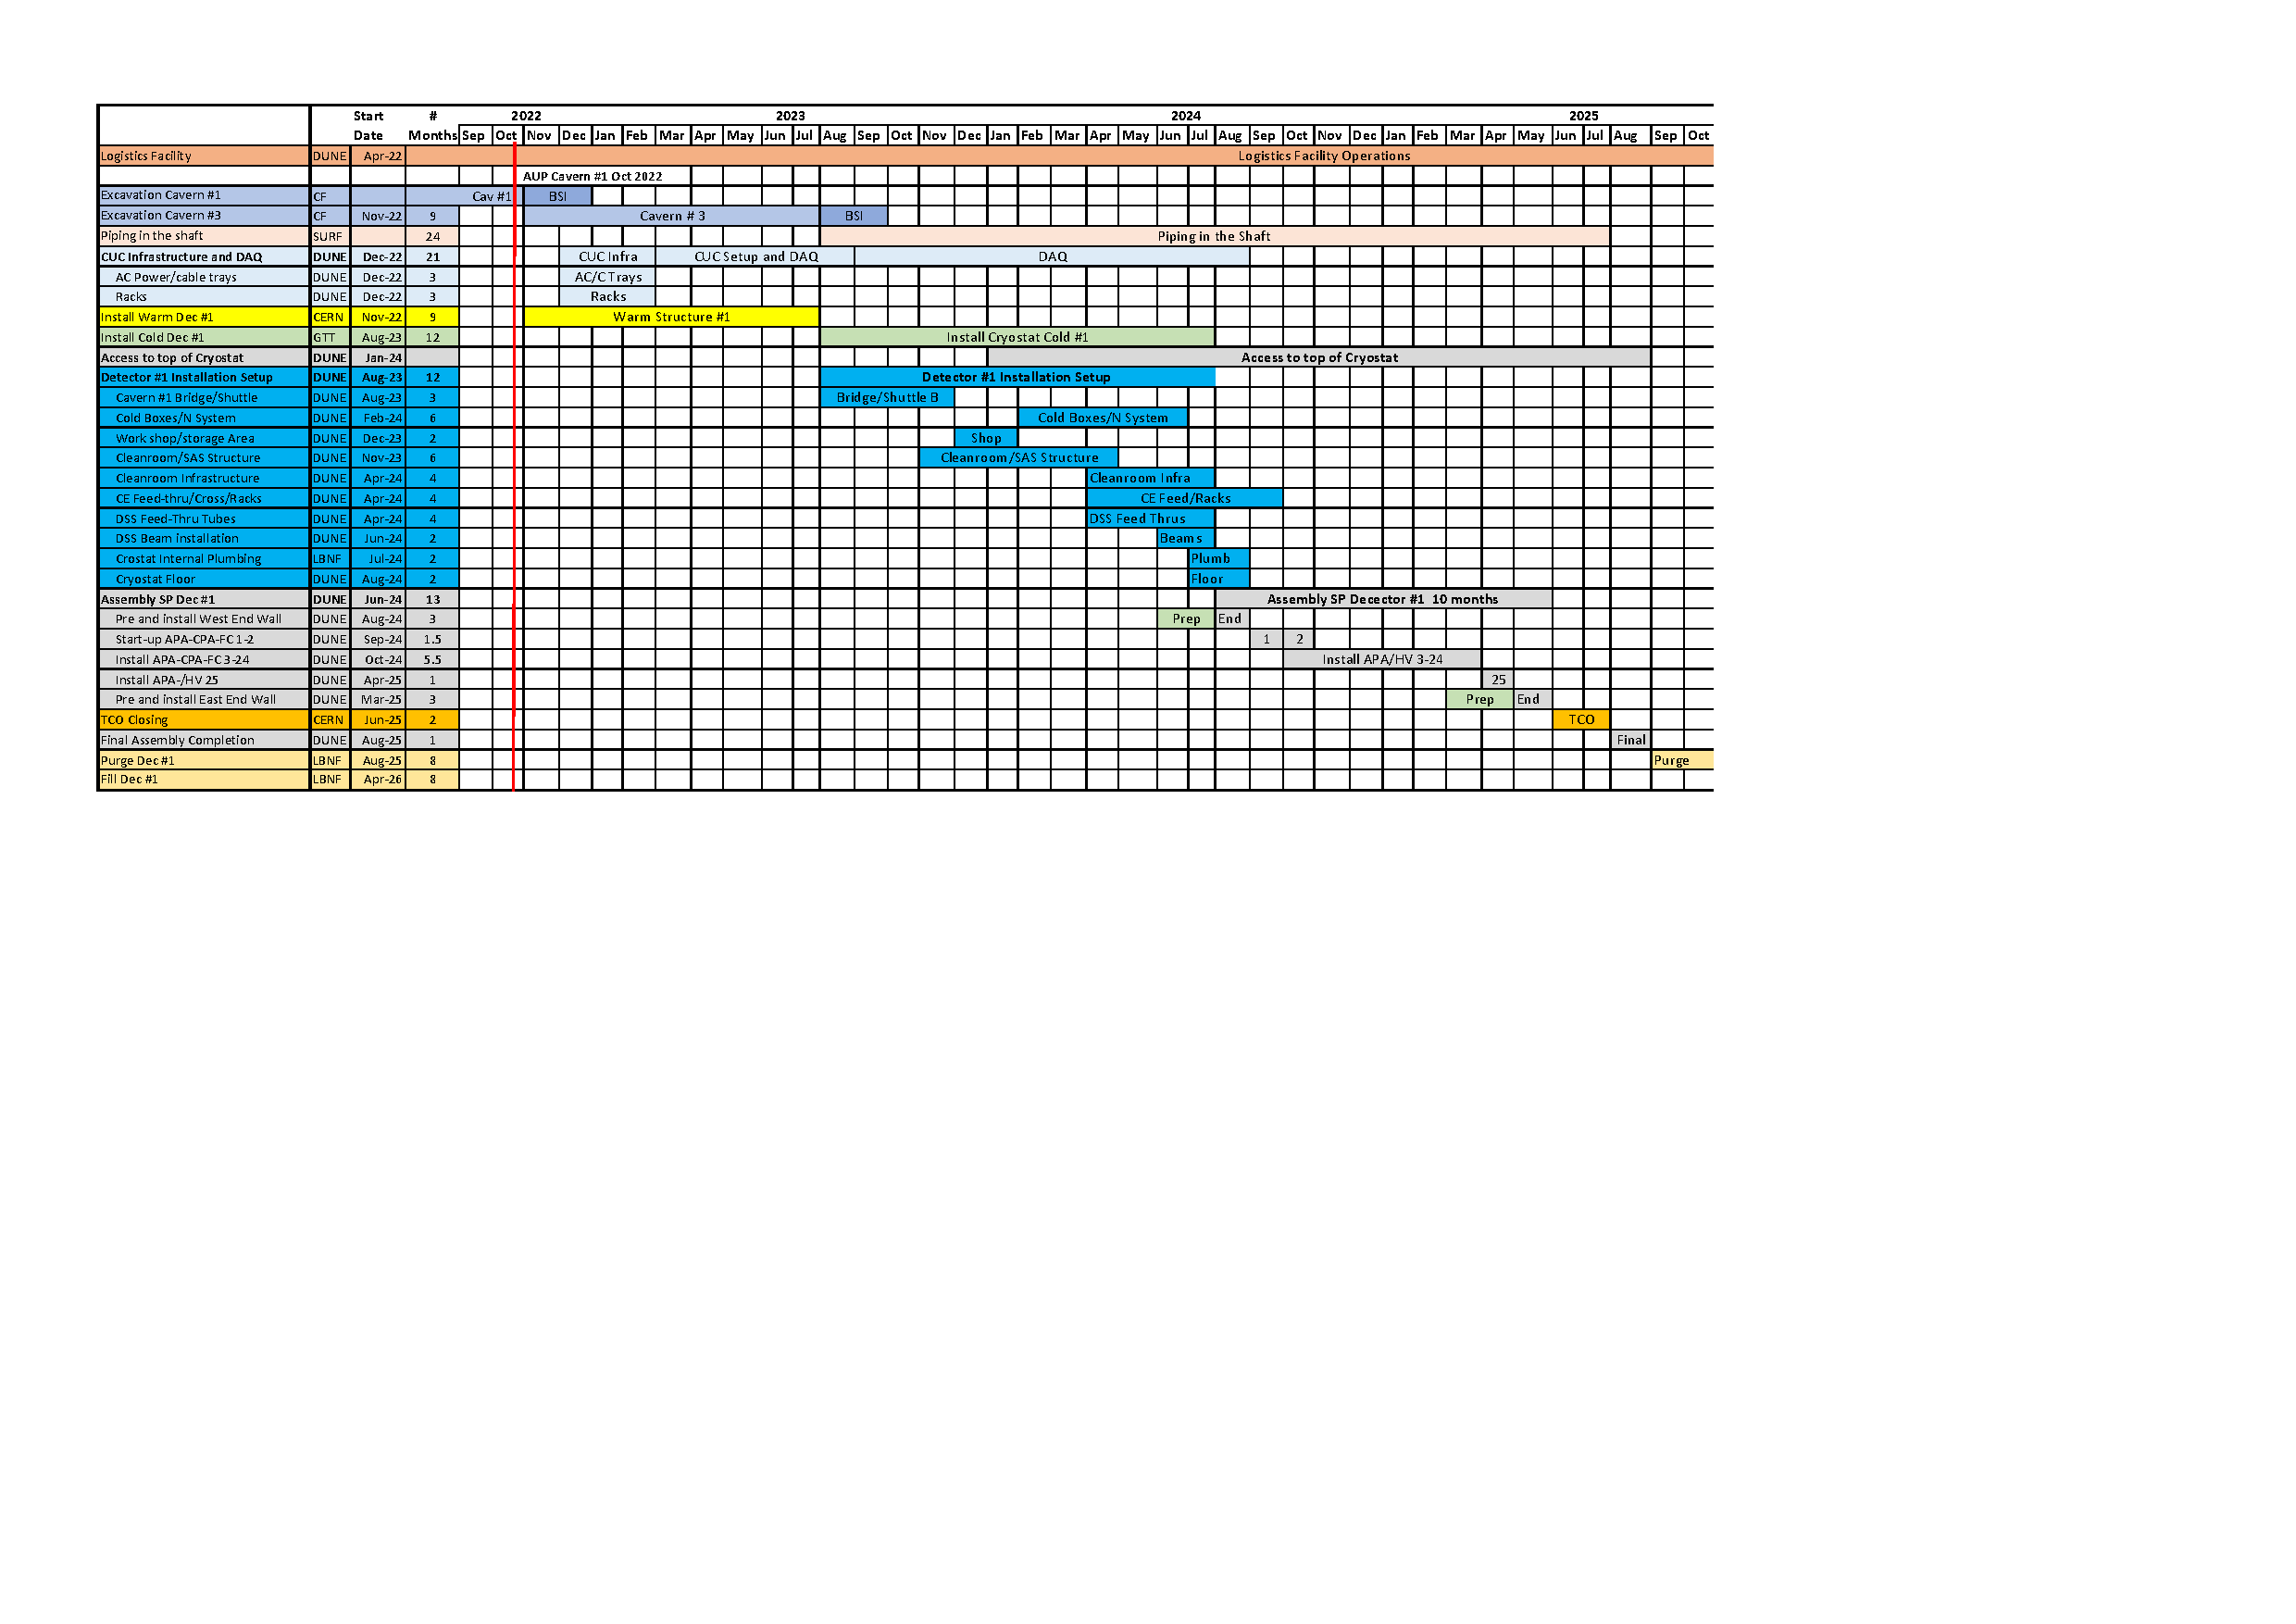
\includegraphics[width=0.98\textwidth]
{Overview-of-SinglePhase-Schedule}
\end{dunefigure}

The cost, schedule, and labor estimates are based on two 10 hour shifts per day, 4 days a week. Work efficiency should be a maximum of 70 percent.  The cage ride takes up approximately 2-3 hours per day, and shift meetings, lunch, coffee breaks, and gowning to go into the cleanroom take more time out of the shift. 

There are three basic schedule phases for Detector 1 installation:

\begin{itemize}
    \item {\bf \dword{cuc} Installation Phase:}
    This period, which is described in detail in section \ref{sec:fdsp-tc-inst-CUC}, can start once \dword{aup} has been received for the north cavern and the \dword{cuc}. This is also the same time that excavation of the south cavern and installation of the warm structure by \dword{lbnf} begins. As no more than 140 \dwords{fte} will be allowed underground at a time,  access to the underground area will be minimal during this period for \dword{dune} personnel.  Work in this period is limited to work inside the \dword{cuc}. Installing the basic rack infrastructure in the dataroom will take an estimated three months, and then installation and testing of the \dword{daq} will continue over the next 12 month period. The \dword{daq} is needed at the start of detector installation.  
    
    \item {\bf Installation Setup Phase:} This phase,  described in detail in section \ref{sec:fdsp-tc-inst-setup}, is when the majority of the infrastructure is installed. During this time, we begin working two shifts per day, and the \dword{uit} team doubles in size.  
    This is a critical training period, so getting lead-workers, riggers, and equipment operators familiar with the tasks is a priority, and adjusting crews to ensure balanced teams.  Before this phase, the \dword{dune} trial assembly equipment at Ash River will be used to begin the training process. During this phase the bridge is constructed along with the coldboxes, the cleanroom and all the equipment in the cleanroom. The \dword{dss} is also installed and surveyed.
    
    \item {\bf Detector Installation Phase:} The final detector installation phase begins with an operational readiness review to check that all documentation and procedures are in place. After the east endwalls are installed, a start-up period of 1.5 months begins for the first two rows of \dword{tpc} components. After that, the installation rate is 9-10 shifts to complete each row.  To meet this schedule, we use two \dword{apa} cabling stations, three coldboxes, and separate crews in the cryostat, all working in parallel.  It will take 5.5 months to install rows 3-24 and about 1 month for row 25. Closing the \dword{tco} will take approximately two months for the cryostat cold structure contractor. During this time, there is no access to the cryostat.  Once this is completed, the final instrumentation is completed, and the purge can begin. 
    
\end{itemize}



\subsection{Detector Commissioning Phase}
\label{sec:fdsp-tc-inst-comiss}
% Anne reviewing this section 3/20/19
%After the \dword{detmodule} is installed in the cryostat, much work remains before it can be operated. First the \dword{tco} must be closed. This requires bringing back the cryostat manufacturer. First the missing panel with steel beams and steel panel are installed to complete the cryostat's outer structural hull. Then the remaining foam blocks and membrane panelsare installed from the inside using the roof access holes to enter the cryostat. 
After the \dword{spmod} is installed in the cryostat, much work remains before it can be operated. 
The cryostat manufacturer must come back to close the \dword{tco}. 
First they install the missing panel %with steel beams and steel panel are installed 
to close it, which completes the cryostat's outer structural hull.  \fixme{correct?} 
Then the remaining foam blocks and membrane panels
are brought inside the cryostat  through the roof's access holes and installed. 


%In parallel, the \lar pumps are installed at the ends of the cryostat and final connections are made to the recirculation plant. Once the pumps are installed, the cryostat is closed, everything is leak tested, and the cryogenics plant can be brought into operation. First the air inside the cryostat is purged by injecting pure argon gas at the bottom  at a rate that fills the cryostat volume uniformly but faster than the diffusionrate. This produces a column of argon gas that rises through the volume and sweeps out the air. This process is referred to as the \textit{piston purge}. When the piston purge is complete, the cool down of the \dword{detmodule} can begin. Misting nozzles inject a liquid-gas mix into the cryostatthat cools the detector components at a controlled rate. 
In parallel, the \lar pumps are installed at the ends of the cryostat and final connections are made to the recirculation plant. Next, everything is leak tested, and the cryogenics plant can be brought into operation. The system first purges the air inside the cryostat  by injecting pure \dword{gar} at the bottom  at a rate that fills the cryostat volume uniformly but faster than the diffusion rate. This ``piston purge'' process produces a column of \dword{gar}  that rises through the volume and pushes out the air.  When the piston purge is complete, misting nozzles inject a liquid-gas mix into the cryostat that cools the detector components at a controlled rate. 

%Once the detector is cold, the filling process can begin. Liquid argon stored at the surface  at \surf is vaporized and brought down the shaft in gaseous form. The gas is then re-condensed underground. The \lar then flows through filters to remove any H$_2$O or O$_2$ and into the cryostat.Given the very large volume of the cryostat and the limited cooling power for recondensing, \num{12} months will be required to fill the first \dword{detmodule}. %During this time
Once the detector is cold, the filling process begins. \dword{lar} stored at the surface  at \dword{surf} is vaporized, brought down the shaft in gaseous form, and re-condensed underground. The \lar then flows through filters to remove any H$_2$O and O$_2$ before entering the cryostat. Given the volume of the cryostat and the limited cooling power for recondensing, \num{12} months will be required to fill the first \dword{detmodule}. the detector readout electronics will be on monitoring the status of the detector. 

Testing and constant monitoring of the detector will take place from \dword{tco} closing until the end of the filling process. 
Before the last %man
access hole is sealed:
\begin{enumerate}

    \item A pedestal and \dword{rms} characterization of all cold electronic channels will verify that all \dword{apa} front-end boards are responding and no dead channel or new noise sources arose following the \dword{tco} closing.
    
    \item A noise scan of all \dword{pd} channels is performed as last check before sealing.

    \item Each \dword{apa} wireplane will be checked to verify it is isolated from the \dword{apa} frame and properly connected to its \dword{hv} power supply through the following steps:
    
\begin{itemize}

    \item The \dword{shv} connector of each wireplane bias channel will be unplugged at the power supply, and the resistance  between inner conductor and ground and its capacitance 
    \fixme{capac betw inner cond and grd? or of sthg else?} will be measured. The resistance should show the wireplane is electrically isolated from the ground, while the capacitance value should match that of the cold \dword{hv} cable and the capacitance of the circuit on the \dword{apa} top frame.

    \item \SI{50}{V} is applied to each wireplane and the current drawn checked against the expected value.
    
    \item Nominal voltages are applied to each wireplane, and the current drawn is checked against the expected value. 
    
\end{itemize}

    \item A low \dword{hv} (i.e., \SIrange{1}{2}{kV}) is applied to the cathode, and the current drawn is checked against the expected value to ensure the integrity of the \dword{hv} line.

\end{enumerate}

During the piston purge process %phase, 
periodic monitoring of %both 
\dword{apa}, \dword{ce}, and \dword{pd} system noise (pedestal, \dword{rms}) will occur.

A number of %these 
the following tests, in addition to new ones, will instead take place during the cool-down phase:

\begin{enumerate}


    \item Each \dword{apa} wireplane isolation and proper connection to its \dword{hv} power supply will be checked at regular time intervals as was done before sealing the cryostat.
    
    \item \SIrange{1}{2}{kV} will be held on the cathode, and the current drawn will be  monitored constantly to observe the trend in temperature of the total resistance.
    
    \item \dword{ce} noise figures (pedestal, \dword{rms}) will be measured at regular intervals and their trends with temperature recorded.
    
    \item \dword{pd} system noise (pedestal, \dword{rms}) will be measured at regular intervals and its trend with temperature recorded.
    
     \item Values of the temperature sensors deployed in several parts of the cryostat will be monitored constantly to %see 
     watch the progress of the cool down phase and to relate the temperature to the behavior of the other \dword{spmod} subsystems. 
     
\end{enumerate}

Regular monitoring of \dword{ce} and \dword{pd} noise, as well as checks of wireplane isolation and proper connections to the bias supply system will continue throughout the filling, recording noise variations as a function of the progressively reduced temperature. In addition,

\begin{enumerate}

    \item As each purity monitor is submerged in liquid, it will be turned on every eight hours to control \dword{lar} purity.
    
    \item As soon as top ground planes are submerged, \dword{hv} on the cathode will be raised up to \SI{10}{V} to check that the current drawn by the system agrees with expectations.

\end{enumerate}

Once the \dword{detmodule} is full, the drift \dword{hv} will be carefully ramped up following these steps:

\begin{enumerate}

    \item The need for a filter regeneration is evaluated before starting any operation;

    \item Once filter regeneration is completed (if needed), the \dword{lar} surface is examined using cameras to verify that the surface is flat, with no bubbles or turbulence;
    
    \item \dword{lar} recirculation is started, and \dword{lar} surface is examined again to see if activating the recirculation system introduced any turbulence into the liquid;
    
    \item Wait one day after beginning  recirculation to stabilize the \dword{lar} flow inside the \dword{detmodule}, then start the \dword{hv} ramp up.
    
\end{enumerate}

Cathode voltage is raised in steps over three days. 
On the first day, cathode voltage is first raised to \SI{60}{kV}, then to \SI{90}{kV} after waiting two hours, and finally to \SI{120}{kV} after waiting another two hours, and then left at this value overnight.
On the second day, cathode voltage is first raised to \SI{140}{kV}, then to \SI{160}{kV} after waiting four hours, and then left at this value overnight. 
On the third day, cathode voltage is first raised to \SI{170}{kV} and then to the nominal operating voltage of \SI{180}{kV} after waiting four hours. 
During each \dword{hv} ramp up, all \dword{ce} current draws are monitored, and the procedure is stopped if any of the current draws go out of the allowed range. 
During each waiting period, regular \dword{daq} runs monitor \dword{ce} and \dword{pd} noise and response, while cathode \dword{hv} and current draw stability are constantly monitored.

In \dword{pdsp}, this process took three days, after which the system was  ready for data-taking. With a detector twenty times larger, the process will take longer, but the turn on time should still be relatively short. 

\subsection{Risks}


% risk table values for subsystem SP-FD-JPO
\begin{longtable}{p{0.15\textwidth}p{0.13\textwidth}p{0.13\textwidth}p{0.28\textwidth}p{0.06\textwidth}p{0.06\textwidth}p{0.06\textwidth}} 
\caption{Specification for SP-FD-JPO \fixmehl{ref \texttt{tab:specs:SP-FD-JPO}}} \\
\rowcolor{dunesky}
ID & Risk & Label & Mitigation & Prob ability & Cost Impact & Sched ule Impact \\  \colhline
RT-JPO-001 & Personnel injury & jpo-person-injury & Follow established safety plans. & M & L & H \\  \colhline
RT-JPO-002 & Shipping delays & jpo-shipping-delay & Plan one month buffer to store  materials locally. Provide logistics manual. & H & L & L \\  \colhline
RT-JPO-003 & Missing components cause delays & jpo-missing-components & Use detailed inventory system to verify availability of  necessary components.  & H & L & L \\  \colhline
RT-JPO-004 & Import, export, visa issues  & jpo-import-visa & Dedicated \dword{fnal} \dword{sdsd}division will expedite import/export and visa-related issues. & H & M & M \\  \colhline
RT-JPO-005 & Lack of available labor  & jpo-labor-avail & Hire early and use Ash River setup to train \dword{jpo} crew. & L & L & L \\  \colhline
RT-JPO-006 & Parts do not fit together & jpo-cannot-assemble & Generate \threed model, create interface drawings, and prototype detector assembly. & H & L & L \\  \colhline
RT-JPO-007 & Cryostat damage & jpo-cryostat-damage & Use cryostat false floor and temporary protection. & L & L & M \\  \colhline
RT-JPO-008 & Weather closes SURF & jpo-weather-delay & Plan for \dword{surf} weather closures & H & L & L \\  \colhline
RT-JPO-009 & Detector failure during \cooldown & jpo-cooldown-failure & Cold test individual components then cold test \dword{apa} assemblies immediately before installation. & L & H & H \\  \colhline

\label{tab:risks:SP-FD-JPO}
\end{longtable}